\documentclass[oneside,final,14pt]{extarticle}
\usepackage[utf8]{inputenc}
\usepackage[english, russian]{babel}
\usepackage{vmargin}
\setpapersize{A4}
\setmarginsrb{2cm}{1.5cm}{1cm}{1.5cm}{0pt}{0mm}{0pt}{13mm}
\usepackage{indentfirst}
\setlength\parindent{1.25cm}

% шрифт Times New Roman
\usepackage{tempora}
\usepackage{newtxmath}

% межстрочный интервал
\usepackage[onehalfspacing]{setspace}

% Для вставки рисунокв
\usepackage{graphicx}

\sloppy

\begin{document}
    \thispagestyle{empty}
    \begin{center}
        \begin{bfseries}
            \MakeUppercase{Министерство цифрового развития, связи и \\
            массовых коммуникаций Российской федерации}\par
            \bigskip
            Ордена Трудового Красного Знамени федеральное государственное \\
            бюджетное образовательное учреждение высшего образования\par
            \bigskip
            \MakeUppercase{"<Московский Технический Университет Связи И\\Информатики">}\par
            \bigskip
            (МТУСИ)\par\bigskip
        \end{bfseries}
        Кафедра "<Информационная безопасность">\par\bigskip\bigskip
        Отчет по практическим занятиям\parпо дисциплине:\par
        "<Технологии программной защиты в Интернете">\par
        на тему:\par"<Panda Internet Security">\par\bigskip
    \end{center}
    \begin{flushright}
        Выполнил студент\\группы БПЗ 1802\\ Гусев Р.М.\par
        \bigskip
        Проверил:\\Осин А.В.
    \end{flushright}
    \vspace*{\fill}
    { \center Москва, 2022}
    \pagebreak

    \tableofcontents
    \addcontentsline{toc}{section}{Введение} %\protect\numberline{}

    \pagebreak

    \section*{Введение}
    В данной работе будет рассмотрен современный антивирус Panda Internet Security, применяющий
    технологии облачных вычислений, искуственного интеллекта и пр. для обнаружения зловредного ПО,
    и проактивную технологию TruePrevent для защиты устройства от оного.\par

    Производителем является компания Panda Security CL, бывшая Panda Software, компания, работающая
    в сфере компьютерной безопасности, основана в 1990 году бывшим руководителем Panda Микелем 
    Уризарбаррена (Mikel Urizarbarrena) в городе Бильбао, что в Испании. Первоначально компания была
    ориентирована на производство антивирусного программного обеспечения, впоследствии она расширила
    линейку своих продуктов за счет приложений, включающих в себя файервол, приложений по обнаружению
    спама и шпионского ПО, технологии по предотвращению киберпреступлений, а также других систем
    управления и утилит безопасности для домашних и корпоративных пользователей.\par

    Существуют версии антивирусного ПО для устройств на основе ОС Windows, OS X, Android и iOS.
    \pagebreak

    \section{История создания и развития антивируса}
    \subsection{История компании}
        Основанная в испанском городе Бильбао в 1990 году Микелем Уризарбаррена, компания первые 17 лет
        просуществовала под именем Panda Software. В 1995 году компания стала лидером на антивирусном рынке
        Испании, а в 1996 году начала свою международную экспансию. На текущий момент компания имеет коммерческие
        представительства в 56 странах мира. В 2007 году началась новая эра компании, в рамках которой она
        намерена консолидировать свои усилия на международном рынке. Во-первых, произошла смена брэнда, и
        теперь компания называется Panda Security, что более четко соответствует предоставлению действительно
        глобальной безопасности. Более того, в уставной капитал компании вошли известные инвестиционные группы:
        сначала Investindustrial и Gala Capital, а затем HarbourVest и Atlantic Bridge. С тех пор компания
        выкупила восемь национальных представительств, работающих по схеме франшизы на ключевых рынках, и
        выпустила на рынок первый полностью «облачный» антивирус. Panda Security в этом году празднует свое
        20-летие.
    \subsection{Продукты и решения}
        Panda Security имеет несколько продуктовых линеек, для домашних и корпоративных пользователей: ПО
        безопасности, устройства безопасности и управляемые сервисы безопасности. Компания также выпустила
        первый антивирус, позволяющий предложить защиту из «облака» (Panda Cloud Antivirus). Все наши решения
        сопровождаются технической поддержкой, состоящей из экспертной команды профессионалов, доступных
        круглосуточно.
    \subsection{Последние достижения в технологиях и инновациях}
        Корпоративный слоган Panda Security, На шаг впереди (One step ahead), показывает ее конкурентное преимущество,
        которое характеризует компанию с первых дней ее существования — ее стремление к постоянным
        инновациям и изменениям, способность быть всегда на шаг впереди в борьбе с компьютерными угрозами.
        \begin{itemize}
            \item {\bf 2009:} Panda Security выпустила первый в истории антивирус, предлагающий защиту из
            «облака», Panda Cloud Antivirus (www.cloudantivirus.com). Данное решение для домашних пользователей
            позиционирует компанию как технологического лидера в данном новом секторе;
            \item {\bf 2008:} Выпуск новой линейки домашних продуктов, предлагающей гибридную систему защиты:
            комбинацию традиционной защиты, основанной на сигнатурном методе обнаружения, с защитой из «облака», 
            усиленной базой знаний Коллективного разума;
            \item {\bf 2007:} Внедрение и выпуск на рынок первой системы Коллективного разума: «облачные»
            технологии способны автоматически классифицировать, анализировать и дезинфицировать тысячи образцов
            новых вредоносных программ, поступающих каждый день в нашу антивирусную лабораторию PandaLabs. Это
            позволяет компании отвечать на вызов со стороны новых угроз в режиме реального времени, в то время
            как другие производители решений безопасности тратят на это несколько дней.
            \item {\bf 2005:} Выпуск нового решения класса SaaS (Security-as-a-Service, Безопасность как сервис),
            Panda WebAdmin;
            \item {\bf 2004:} Запуск первой Хост-ориентированной системы предотвращения вторжений (Host Intrusion
            Prevention System, HIPS) для всех типов компьютеров, рабочих станций или домашних ПК, с технологиями
            TruPrevent® и собственным модулем поведенческого анализа.
        \end{itemize}
    \pagebreak

    \section{Системные требования}
        Для ОС Windows:\par
        Операционная система: 
        \begin{itemize}
    
            \item Windows 7 (32 и 64-bit);
            \item Windows Vista (32 и 64-bit);
            \item Windows XP 32-bit;
            \item И поздние версии;
        \end{itemize}
        Процессор: Intel Atom, Intel Celeron M, VIA C7-M\par
            ОЗУ: 
        \begin{itemize}
            \item 128 МБ без TruPrevent 
            \item 512 МБ с TruPrevent (рекомендуется 1 ГБ) 
        \end{itemize}
            Жесткий диск: 265 МБ свободного пространства\par
            MS Internet Explorer 6.0\par
            
            Для активации продукта требуется наличие Интернет-соединения\par
    \pagebreak

    \section{Обзор функционала}
        Обзор антивирусного ПО Panda Security будет проходить на ОС Windows 10 x64, при наличии 32 Гб оперативнгй памяти.\par
        Сравнение тарифных планов приведено на \ref{tariff_compare}.\par
        \begin{figure}[h]
            \centering
            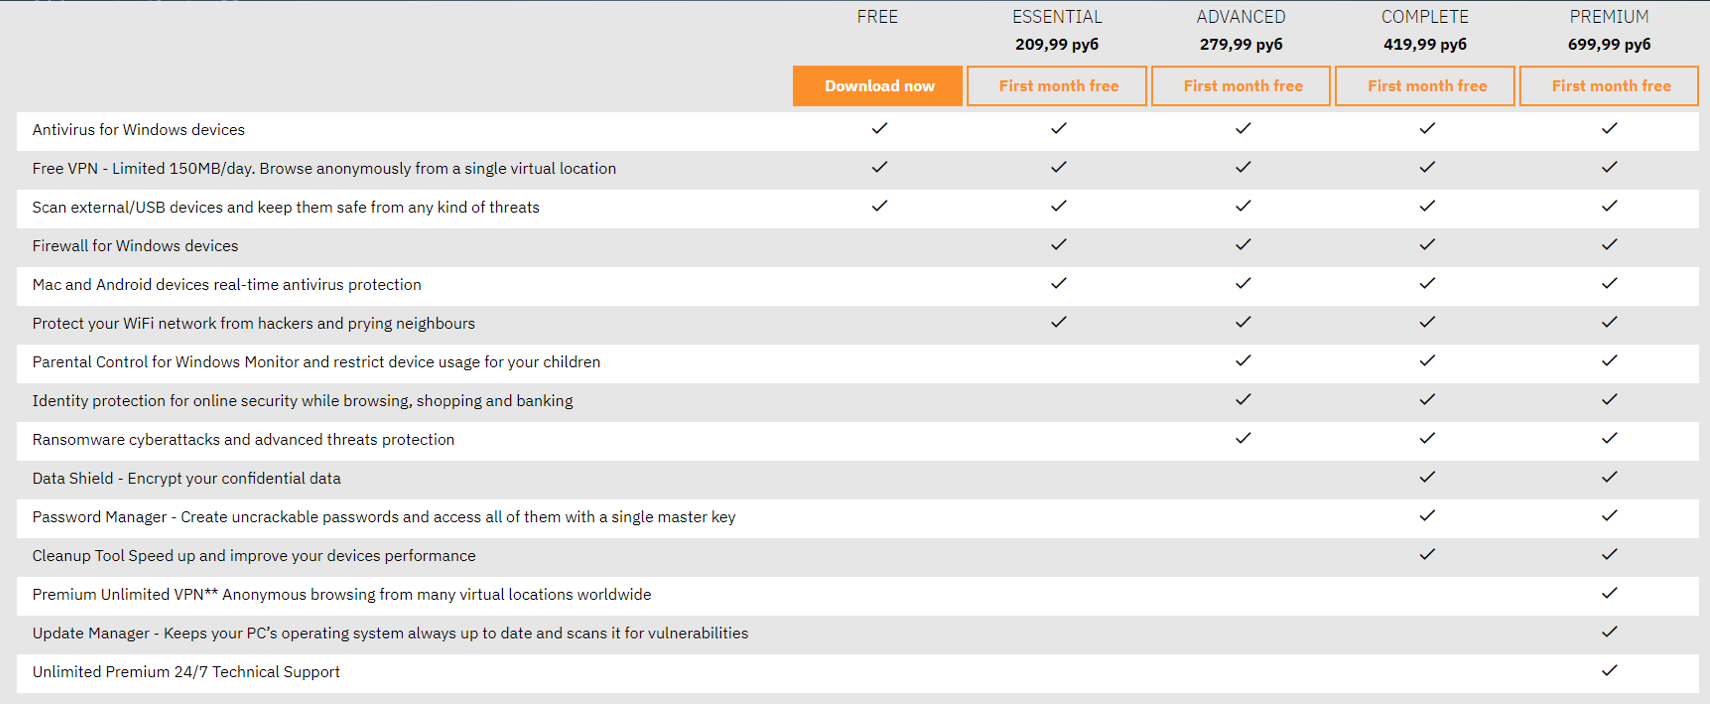
\includegraphics[width=\textwidth]{pics/compare_tariffs}
            \caption{Сравнение тарифных планов}
            \label{tariff_compare}
        \end{figure}
        В бесплатную версию антивируса входит антивирус для ОС Windows, модуль антивируса для мобильной ОС
        Android, сканер USB-носителей, а так же VPN, ограниченный 150 МБ/день и сканер Panda Cloud Cleaner,
        применяющий технологию облачных вычислений и ИИ "<Коллективный разум"> при этих самых вычислениях.\par
        Тариф антивируса \emph{Essential} включает в себя все модули бесплатного тарифа, а также фаервол для 
        ОС Windows, антивирусную защиту для устройств Mac и защиту Wi-Fi сети от взломщиков и соседей.\par
        Тариф \emph{Advanced} включает в себя все модули вышеуказанных тарифов, а также включает в себя
        модуль родительского контроля, который можно также докупить отдельно для более дешевых тарифных планов,
        конфиденциальность и защиту при интернет-шоппинге, банкинге и т.д., а так же защиту от более сложного
        зловредного ПО.\par
        Тариф \emph{Complete} помимо всех вышеупомянутых модулей включает в себя модуль шифрования конфиденциалных
        данных, менеджер паролей и утилиту очистки устройства, которая может позволить увеличить производительность
        устройства.\par
        И наконец, самый полный тариф, \emph{Premium}, включает в себя так же безлимитный VPN, менеджер 
        обновлений операционной системы и безлимитную Premium 24/7 службу поддержки.
    \pagebreak

    \section{Главное окно приложения}
    \pagebreak

    \section{Параметры}
    \pagebreak

    \section{Тестирование}
    \pagebreak

    \section{Преимущества и недостатки}
    \pagebreak

    \section*{Заключение}
    \pagebreak

\end{document}